%\documentclass[draft]{ua-thesis}
\documentclass[final]{ua-thesis}
%<my packages>
%% Language and font encodings
\usepackage{gb4e}
\noautomath
\usepackage{natbib}
\usepackage[english]{babel}
\usepackage[utf8x]{inputenc}
\usepackage[T1]{fontenc}

%% Sets page size and margins
%\usepackage[a4paper,top=3cm,bottom=2cm,left=3cm,right=3cm,marginparwidth=1.75cm]{geometry}

%% Useful packages
\usepackage{amsmath}
\usepackage{graphicx}
\usepackage[colorinlistoftodos]{todonotes}
\usepackage[colorlinks=true, allcolors=blue]{hyperref}
\usepackage{fixltx2e}
\usepackage{Sweave}

\newcommand*{\myfont}{\fontfamily{ccr}\selectfont}
%the newcommand change the selected word into 'ccr' font
%e.g. \begin{myfont} multi-bleu.perl \end{myfont}
%\<my packages>


\usepackage{verbatim}
%\usepackage{amssymb,amsmath,amsthm}
%\usepackage[mathscr]{eucal}

\usepackage{makeidx}
\numberwithin{equation}{section}
%\numberwithin{equation}{subsection}
%%====================================================================
%-------------------------------------------------------------------- 
%
%   isomath.tex  LaTeX macros for math conforming to ISO standards
%
%---------------------------------------- this is a LaTeX-2e document
%====================================================================     

%% Blackboard Bold

\newcommand*{\bbb}[1]{\mathbb{#1}}
\newcommand{\bC}{\bbb{C}}
\newcommand{\bN}{\bbb{N}}
\newcommand{\bQ}{\bbb{Q}}
\newcommand{\bR}{\bbb{R}}
\newcommand{\bZ}{\bbb{Z}}
\newcommand{\bF}{\bbb{F}}
\newcommand{\bFp}{\bbb{F}_p}
\newcommand{\bFpn}{\bbb{F}_{p^n}}
\newcommand{\ii}{\mathbf{i}}
\newcommand{\jj}{\mathbf{j}}
\newcommand{\kk}{\mathbf{k}}

\newcommand{\N}{\bN}
\newcommand{\Q}{\bQ}
\newcommand{\R}{\bR}
\newcommand{\Z}{\bZ}
\newcommand{\ZpZ}{\Z/p\Z}
\newcommand{\ZmZ}{\Z/m\Z}
\newcommand{\C}{\bC}
%\newcommand{\F}{\bF}
\newcommand{\F}{\mathbb{F}}
\newcommand{\Fp}{\bFp}
\newcommand{\Fpn}{\bFpn}

%% Calligraphic

\newcommand{\mC}{\mathcal{C}}
\newcommand{\mT}{\mathcal{T}}

%% Miscellaneous

%% Named Functions and Operators

\newcommand{\id}{\mathrm{id}}
\newcommand{\Id}{\mathrm{Id}}
\newcommand{\rank}{\mathrm{rank}}
\newcommand{\supp}{\mathrm{supp}}
\newcommand{\tr}{\mathrm{tr}}
\newcommand{\Aut}{\mathrm{Aut}}
\newcommand{\Gal}{\mathrm{Gal}}
\newcommand{\Hom}{\mathrm{Hom}}
\newcommand{\im}{\mathrm{im}}
\newcommand{\lcm}{\mathrm{lcm}}
\newcommand{\Tr}{\mathrm{Tr}}
\newcommand{\GL}{\mathrm{GL}}
%\newcommand{\mod}{\textrm{ mod }}

%% Vectors

\usepackage{amsbsy}
\renewcommand*{\vec}[1]{\boldsymbol{#1}}
\newcommand{\va}{\vec{a}}
\newcommand{\vb}{\vec{b}}
\newcommand{\vc}{\vec{c}}
\newcommand{\vx}{\vec{x}}
\newcommand{\vy}{\vec{y}}
\newcommand{\vz}{\vec{z}}
\newcommand{\vu}{\vec{u}}
\newcommand{\vv}{\vec{v}}
\newcommand{\vw}{\vec{w}}

%% Logical Propositions

\newcommand*{\pro}[1]{\mathsf{#1}}
\newcommand{\pP}{\pro{P}}
\newcommand{\pQ}{\pro{Q}}
\newcommand{\pR}{\pro{R}}

%% Matrices and Tensors

%\DeclareMathAlphabet{\mathsfsl}{OT1}{cmss}{m}{sl}
\newcommand*{\mat}[1]{\mathsfsl{#1}}
\newcommand{\mM}{\mat{M}}
\newcommand{\mD}{\mat{D}}
\newcommand{\mI}{\mat{I}}

%% Special Numbers and Characters

\newcommand{\re}{\mathrm{e}}
\newcommand{\ri}{\mathrm{i}}
\newcommand{\rd}{\mathrm{d}} % differential
\newcommand{\dif}[1]{\,\rd{#1}} % differential
\newcommand{\df}{\dif{f}}
\newcommand{\dx}{\dif{x}}
\newcommand{\dy}{\dif{y}}
\newcommand{\dz}{\dif{z}}
\newcommand{\dt}{\dif{t}}
\newcommand{\rpi}{\pi}       % actually, pi should be upright.

\newcommand{\rE}{\mathsf{E}}
\newcommand{\rF}{\mathsf{F}}
\newcommand{\rI}{\mathsf{I}}
\newcommand{\rK}{\mathsf{K}}
\newcommand{\rL}{\mathsf{L}}
\newcommand{\rM}{\mathsf{M}}
\newcommand{\rN}{\mathsf{N}}
\newcommand{\rP}{\mathsf{P}}
\newcommand{\rT}{\mathsf{T}}
\newcommand{\rU}{\mathsf{U}}
\newcommand{\rV}{\mathsf{V}}
\newcommand{\rW}{\mathsf{W}}
\newcommand{\rX}{\mathsf{X}}
\newcommand{\rY}{\mathsf{Y}}
\newcommand{\rZ}{\mathsf{Z}}

%====================================================================
%
%  mathenv.tex  math environments  version 0.00
%
%====================================================================

\usepackage{ifthen}

\theoremstyle{plain}
%\newtheorem{thm}{Theorem}[subsection]
\newtheorem{thm}[equation]{Theorem}
\newtheorem{cor}[equation]{Corollary}
\newtheorem{lem}[equation]{Lemma}
\newtheorem{prop}[equation]{Proposition}
\newtheorem{ax}[equation]{Axiom}
\newtheorem*{thm*}{Theorem}
\newtheorem*{cor*}{Corollary}
\newtheorem*{lem*}{Lemma}
\newtheorem*{prop*}{Proposition}
\newtheorem*{ax*}{Axiom}

\theoremstyle{definition}
\newtheorem{defn}[equation]{Definition}
\newtheorem{problem}{Problem}
\newtheorem*{defn*}{Definition}
\newtheorem*{problem*}{Problem}
% \newtheorem{ex}[equation]{Example}
% \newtheorem{exs}[equation]{Examples}
% \newtheorem*{ex*}{Example}
% \newtheorem*{exs*}{Examples}

%\theoremstyle{remark}
\newtheorem{rem}[equation]{Remark}
\newtheorem*{rem*}{Remark}
\newtheorem{aside}[equation]{Aside}
\newtheorem*{aside*}{Aside}
\newtheorem{intuition}[equation]{Intuition}
\newtheorem*{intuition*}{Intuition}
\newtheorem{notn}[equation]{Notation}
\newtheorem*{notn*}{Notation}
\newtheorem{conv}[equation]{Convention}
\newtheorem*{conv*}{Convention}
\newtheorem{interp}[equation]{Interpretation}
\newtheorem*{interp*}{Interpretation}
\newtheorem{mnem}[equation]{Mnemonic}
\newtheorem*{mnem*}{Mnemonic}
\newtheorem{exer}[equation]{Exercise}
\newtheorem*{exer*}{Exercise}
\newtheorem{conjecture}[equation]{Conjecture}
\newtheorem*{conjecture*}{Conjecture}

%\numberwithin{equation}{subsection}
%\numberwithin{equation}{section}

%\newcommand{\beginex}{\begin{ex}$\blacktriangleright$ }
%\newcommand{\mendex}{\hfill$\blacktriangleleft$\end{ex}}
\newcommand{\beginex}{\begin{ex}$\rhd$ }
\newcommand{\mendex}{\hfill$\lhd$\end{ex}}

%--------------------------------------------------------------------
%
%\newenvironment{problem}[1][]
% {\noindent{\bf#1.\ }}
% {}
%
%--------------------------------------------------------------------

\newenvironment{answer}[1][Answer]
  {\begin{proof}[#1]}
  {\renewcommand{\qedsymbol}{}\end{proof}}

\newenvironment{solution}[1][Solution]
  {\begin{proof}[#1]}
  {\renewcommand{\qedsymbol}{\ensuremath{\Diamond}}\end{proof}}

\newcounter{ppart}
\newenvironment{parts}
 {\begin{list}{\textup(\alph{ppart}\textup)\hfill}
   {\usecounter{ppart}
    \settowidth{\labelwidth}{\textup(m\textup)}
    \setlength{\leftmargin}{0cm} 
    \setlength{\rightmargin}{0cm}
    \setlength{\itemindent}{2em}
    \setlength{\labelsep}{\itemindent}
    \addtolength{\labelsep}{-\labelwidth}
    \renewcommand{\makelabel}[1]{\ifthenelse
     {\equal{##1}{}}
     {\textup{(\alph{ppart})}\hfill}
     {\textup{##1}\hfill}}
   }
 }
 {\end{list}}

%\renewcommand{\labelenumi}{(\roman{enumi})}

\newcommand{\secref}[1]{Section~\textup{\ref{#1}}}
\newcommand{\thmref}[1]{Theorem~\textup{\ref{#1}}}
\newcommand{\corref}[1]{Corollary~\textup{\ref{#1}}}
\newcommand{\lemref}[1]{Lemma~\textup{\ref{#1}}}
\newcommand{\propref}[1]{Proposition~\textup{\ref{#1}}}
\newcommand{\defnref}[1]{Definition~\textup{\ref{#1}}}
\newcommand{\remref}[1]{Remark~\textup{\ref{#1}}}
\newcommand{\exref}[1]{Example~\textup{\ref{#1}}}
\newcommand{\exsref}[1]{Examples~\textup{\ref{#1}}}
\newcommand{\axref}[1]{Axiom~\textup{\ref{#1}}}
\newcommand{\itemref}[1]{\textup{{\ref{#1}}}}

% Vim 7.0 syntax highlighting doesn't seem to kick in unless the .tex
% file has at least one begin-end pair in it.  Go figure.
\newenvironment{vim_bug_workaround}
	{}

%====================================================================


\newcommand*{\ds}[1]{\displaystyle{#1}}

\newcommand*{\bfidx}[1]{\index{#1}\textbf{#1}}
\newcommand*{\bfidxtwo}[2]{\textbf{#1}\index{#2}}
\newcommand*{\bfidxaux}[2]{\index{#1}\index{#2}\textbf{#1}}
\newcommand*{\emphidx}[1]{\index{#1}\emph{#1}}
\newcommand*{\plainidx}[1]{\index{#1}#1}

\newcommand*{\bra}[1]{\langle \, #1 \mid}
\newcommand*{\ket}[1]{\mid #1 \, \rangle}
\newcommand*{\braket}[2]{\langle #1 \mid #2 \rangle}
\newcommand*{\braCket}[3]{\langle #1 \mid #2 \mid #3 \rangle}
\newcommand*{\BraCKet}[3]
	{\Bigg\langle #1 \,\Bigg|\, #2 \,\Bigg|\, #3 \Bigg\rangle}
\newcommand*{\expn}[1]{\langle \, #1 \, \rangle}
\newcommand*{\ketbra}[1]{\ket{ #1 } \bra{ #1 }}
\newcommand*{\TrebH}{\Tr\left(e^{-\beta H}\right)}
\newcommand*{\TrXebH}[1]{\Tr\left(#1 e^{-\beta H}\right)}
\newcommand*{\Trsym}{\Tr_{L^2_{\mathrm{sym}}}}
\newcommand*{\intRdntimes}[2]{\underbrace{
	\int_{\R^{#1}} \int_{\R^{#1}} \cdots \int_{\R^{#1}}}_{#2 \textrm{ times}}}

\newcommand{\lmax}{\ell_{\textrm{max}}}

\newcommand{\ellx}{\ell_{\vecx}}
\newcommand{\elly}{\ell_{\vecy}}

\newcommand{\ellxpi}{\ell_{\vecx}(\pi)}
\newcommand{\ellypi}{\ell_{\vecy}(\pi)}

\newcommand{\ellxpiprime}{\ell_{\vecx}(\pi')}
\newcommand{\ellypiprime}{\ell_{\vecy}(\pi')}

\newcommand{\ellxypi}{\ell_{\vecx,\vecy}(\pi)}
\newcommand{\ellyxpi}{\ell_{\vecy,\vecx}(\pi)}

\newcommand{\essx}{s_{\vecx}}

\newcommand{\essxpi}{s_{\vecx}(\pi)}

\newcommand{\ellxf}{\ell^f_{\vecx}}
\newcommand{\essxf}{s^f_{\vecx}}
\newcommand{\ellmax}{\ell_{\textrm{max}}}
\newcommand{\fM}{f_{\textrm{max}}}
\newcommand{\ellbar}{\overline{\ell}}
\newcommand{\ellfbar}{\overline{\ell}_f}
\newcommand{\essbar}{\overline{s}}
\newcommand{\essfbar}{\overline{s}_f}

\newcommand{\rhocz}{\rho_c^{(0)}}
\newcommand{\rhocal}{\rho_c^{(\alpha)}}
\newcommand{\betacz}{\beta_c^{(0)}}
\newcommand{\betacal}{\beta_c^{(\alpha)}}
\newcommand{\Tcz}{T_c^{(0)}}
\newcommand{\Tcal}{T_c^{(\alpha)}}

\newcommand{\Xt}{X_t}
\newcommand{\Yt}{Y_t}
\newcommand{\Xtk}{X_{t+k}}
\newcommand{\Ytk}{Y_{t+k}}

\newcommand{\cmhat}{\hat{c}_m}
\newcommand{\chat}{\hat{c}}
\newcommand{\tauint}{{\tau_{\textrm{int}}}}
\newcommand{\hattauint}{\hat{\tau}_{\textrm{int}}}
\newcommand{\tauexp}{{\tau_{\textrm{exp}}}}
\newcommand{\stilde}{{\tilde{s}}}
\newcommand{\ttilde}{{\tilde{t}}}

\newcommand{\sumiB}{\sum_{i=0}^{B-1}}
\newcommand{\sumjB}{\sum_{j=0}^{B-1}}
\newcommand{\sumiM}{\sum_{i=0}^{M-1}}
\newcommand{\sumjM}{\sum_{j=0}^{M-1}}
\newcommand{\sumiN}{\sum_{i=0}^{N-1}}
\newcommand{\sumjN}{\sum_{j=0}^{N-1}}

%% ----------------------------------------------------------------
\def\ve{\varepsilon}
\def\veps{\varepsilon}
\def\bbB{\mathbb{B}}
\def\bbE{\mathbb{E}}
\def\bbP{\mathbb{P}}
\def\muhat{\hat{\mu}}
\def\psihat{\hat{\psi}}
\def\fhat{\hat{f}}
\def\ghat{\hat{g}}
\def\Ahat{\hat{A}}
\def\Fhat{\hat{F}}
\def\Hhat{\hat{H}}
\def\What{\hat{W}}
\def\Yhat{\hat{Y}}
\def\Zhat{\hat{Z}}
\def\nuhat{\hat{\nu}}
\def\rhohat{\hat{\rho}}
\def\Xihat{\hat{Xi}}
\def\xbar{\overline{x}}
%\def\torusdiff{\tilde{\vecd}}
\def\torusdiff{\vecd_\Lambda}

\def\muX{\mu_{X}}
\def\muY{\mu_{Y}}
\def\muXNbar{\mu_{\overline{X}_N}}
\def\muYNbar{\mu_{\overline{Y}_N}}
\def\sigmaX{\sigma_{X}}
\def\sigmaY{\sigma_{Y}}
\def\sigmaXNbar{\sigma_{\overline{X}_N}}
\def\sigmaYNbar{\sigma_{\overline{Y}_N}}

\def\ANbar{{\overline{A}_N}}

\def\QMbar{{\overline{Q}_M}}

\def\Xbar{\overline{X}}
\def\XNbar{{\overline{X}_N}}
\def\XMbar{{\overline{X}_M}}
\def\XNBbar{{\overline{X}_{N,B}}}

\def\Ybar{\overline{Y}}
\def\YNbar{\overline{Y}_N}
\def\YNBbar{\overline{Y}_{N,B}}

\def\Z{\mathbb{Z}}

\def\Htilde{\tilde{H}}
\def\Halpha{H^{(\alpha)}}
\def\HP{H_P}
\def\HPzero{H_P^{(0)}}
\def\HPone{H_P^{(1)}}

\def\bfH{\mathbf{H}}
\def\bfx{\mathbf{x}}

\def\bsH{\mathbf{H}}
\def\bsx{\mathbf{x}}

\def\caS{\mathcal{S}}
\def\mcS{\mathcal{S}}

\def\mcF{\mathcal{F}}
\def\mcK{\mathcal{K}}
\def\mcL{\mathcal{L}}
\def\mcH{\mathcal{H}}
\def\mcN{\mathcal{N}}
\def\mcO{\mathcal{O}}

\def\msH{\mathscr{H}}
\newcommand*{\pig}[1]{\langle #1 \rangle}
\newcommand*{\pigm}[1]{\langle #1 \rangle_M}

%% ----------------------------------------------------------------
\newcommand{\Sn}{\mathcal{S}_n}
\newcommand{\SN}{\mathcal{S}_N}
\newcommand{\SNp}{\mathcal{S}_{N+1}}
\newcommand{\SNpc}{{\SNp \setminus \SN}}
\newcommand{\dd}{\mathrm{d}}
\newcommand{\e}{\mathrm{e}}
\newcommand{\Var}{\mathrm{Var}}
\newcommand{\Corr}{\mathrm{Corr}}
\newcommand{\Cov}{\mathrm{Cov}}

%% ----------------------------------------------------------------
\def\veca{\mathbf{a}}
\def\vecb{\mathbf{b}}
\def\vecc{\mathbf{c}}
\def\vecd{\mathbf{d}}
\def\vecg{\mathbf{g}}
\def\veck{\mathbf{k}}
\def\vecm{\mathbf{m}}
\def\vecn{\mathbf{n}}
\def\vecr{\mathbf{r}}
\def\vecu{\mathbf{u}}
\def\vecv{\mathbf{v}}
\def\vecw{\mathbf{w}}
\def\vecx{\mathbf{x}}
\def\vecy{\mathbf{y}}
\def\vecz{\mathbf{z}}

\def\vecK{\mathbf{K}}
\def\vecM{\mathbf{M}}
\def\vecP{\mathbf{P}}
%\def\vecP{\mathcal{P}}
\def\vecV{\mathbf{V}}
\def\vecW{\mathbf{W}}
\def\vecWhat{\hat{\mathbf{W}}}
\def\vecX{\mathbf{X}}
\def\vecY{\mathbf{Y}}
\def\vecZ{\mathbf{Z}}

\def\vecPpiz{\vecP^{(\pi_0)}}
\def\Ppiz{P^{(\pi_0)}}
\def\P{P_{\mathrm{Gibbs}}}
\def\Phat{\hat{P}_{\mathrm{Gibbs}}}

%\def\mkvM{\mathbf{M}}
%\def\mkvM{R}
\def\mkvM{A}
%\def\mkvM{\mathcal{M}}

\newcommand{\vecomega}{{\boldsymbol{\omega}}}
\newcommand{\vecmu}{{\boldsymbol{\mu}}}
\newcommand{\vecnu}{{\boldsymbol{\nu}}}

\def\vecxi{\mathbf{x}_{i}}
\def\vecxj{\mathbf{x}_{j}}
\def\vecxpii{\mathbf{x}_{\pi(i)}}
\def\vecxpij{\mathbf{x}_{\pi(j)}}
\def\vecxpik{\mathbf{x}_{\pi(k)}}
\def\veckpii{\mathbf{k}_{\pi(i)}}

\def\pii{\pi^{-1}}
\def\piinv{\pi^{-1}}

\def\pix{\pi(\vecx)}
\def\piy{\pi(\vecy)}

\def\piprimex{\pi'(\vecx)}
\def\piprimey{\pi'(\vecy)}

\def\piv{\pi(\vecv)}
\def\piw{\pi(w)}
\def\piiw{\pi^{-1}(w)}
\def\piix{\pi^{-1}(\vecx)}
\def\piiy{\pi^{-1}(\vecy)}
\def\edh{e^{-\Delta H}}

\def\vecwi{\mathbf{w}^{(i)}}
\def\vecwj{\mathbf{w}^{(j)}}
\def\vecwk{\mathbf{w}^{(k)}}
\def\vecwij{\mathbf{w}^{(ij)}}

\def\vecwil{\mathbf{w}^{(i_\ell)}}
\def\vecwjl{\mathbf{w}^{(j_\ell)}}

\def\xhat{\hat{x}}
\def\yhat{\hat{y}}

\DeclareMathOperator*{\ctdto}{\circ\hspace{-0.2mm}--\hspace{-0.3mm}\circ}
\DeclareMathOperator*{\notctdto}{\circ\hspace{-0.2mm}--\hspace{-2.5mm}\not--\hspace{-0.3mm}\circ}
\def\maybeeq{\stackrel{?}{=}}
\DeclareMathOperator*{\twocyc}{\circ\hspace{-0.2mm}-\pi-\hspace{-0.4mm}\circ}
\DeclareMathOperator*{\ntwocyc}{\circ\hspace{-0.2mm}-\not\pi-\hspace{-0.4mm}\circ}


%% ----------------------------------------------------------------
\newcommand{\tand}{\textrm{and}}
\newcommand{\qand}{\quad\textrm{and}\quad}
\newcommand{\qqand}{\qquad\textrm{and}\qquad}
\newcommand{\qor}{\quad\textrm{or}\quad}
\newcommand{\qqor}{\qquad\textrm{or}\qquad}
\newcommand{\qie}{\quad\textrm{i.e.}\quad}
\newcommand{\qqie}{\qquad\textrm{i.e.}\qquad}
\newcommand{\qqwith}{\qquad\textrm{with}\qquad}

%% ================================================================
%\newcommand{\Suto}{S\"ut\H{o}}
\def\Suto{S\"ut\H{o}}

\newcommand{\grad}{\nabla}
\newcommand{\tensor}{\otimes}
\newcommand{\into}{\hookrightarrow}
\newcommand{\longto}{\longrightarrow}
\def\upto{\nearrow}
\newcommand{\ix}{\pi(x)}
\newcommand{\iy}{\pi^{-1}(y)}
\newcommand{\iu}{\pi(u)}
\newcommand{\tat}{\textasciitilde}

\newcommand*{\boxalign}[1]{
	\begin{equation*}
	\addtolength{\fboxsep}{5pt}
	\boxed{
	\begin{aligned}
	#1
	\end{aligned}
	}
	\end{equation*}
}

\newcommand*{\rowvectwo}[2]{\begin{pmatrix}#1 & #2 \end{pmatrix}}
\newcommand*{\rowvecthree}[3]{\begin{pmatrix}#1 & #2 & #3\end{pmatrix}}

\newcommand*{\colvecone}[1]{\left(\begin{array}{r} #1 \end{array}\right)}
\newcommand*{\colvectwo}[2]{\left(\begin{array}{r} #1 \\ #2 \end{array}\right)}
\newcommand*{\colvecthree}[3]{\left(\begin{array}{r} #1 \\ #2 \\ #3\end{array}\right)}
\newcommand*{\colvecfour}[4]{\left(\begin{array}{r} #1 \\ #2 \\ #3 \\ #4\end{array}\right)}

\newcommand*{\collvecone}[1]{\left(\begin{array}{l} #1 \end{array}\right)}
\newcommand*{\collvectwo}[2]{\left(\begin{array}{l} #1 \\ #2 \end{array}\right)}
\newcommand*{\collvecthree}[3]{\left(\begin{array}{l} #1 \\ #2 \\ #3\end{array}\right)}
\newcommand*{\collvecfour}[4]{\left(\begin{array}{l} #1 \\ #2 \\ #3 \\ #4\end{array}\right)}

\newcommand*{\colcvecone}[1]{\left(\begin{array}{c} #1 \end{array}\right)}
\newcommand*{\colcvectwo}[2]{\left(\begin{array}{c} #1 \\ #2 \end{array}\right)}
\newcommand*{\colcvecthree}[3]{\left(\begin{array}{c} #1 \\ #2 \\ #3\end{array}\right)}
\newcommand*{\colcvecfour}[4]{\left(\begin{array}{c} #1 \\ #2 \\ #3 \\ #4\end{array}\right)}

\newcommand*{\colrvecone}[1]{\left(\begin{array}{r} #1 \end{array}\right)}
\newcommand*{\colrvectwo}[2]{\left(\begin{array}{r} #1 \\ #2 \end{array}\right)}
\newcommand*{\colrvecthree}[3]{\left(\begin{array}{r} #1 \\ #2 \\ #3\end{array}\right)}
\newcommand*{\colrvecfour}[4]{\left(\begin{array}{r} #1 \\ #2 \\ #3 \\ #4\end{array}\right)}

%% ----------------------------------------------------------------
\newcommand{\D}{\partial}
\newcommand{\DA}{\partial A}
\newcommand{\DB}{\partial B}
\newcommand{\DC}{\partial C}
\newcommand{\DX}{\partial X}
\newcommand{\Dc}{\partial c}
\newcommand{\Df}{\partial f}
\newcommand{\Dg}{\partial g}
\newcommand{\DG}{\partial G}
\newcommand{\Dh}{\partial h}
\newcommand{\DM}{\partial M}
\newcommand{\Dr}{\partial r}
\newcommand{\Du}{\partial u}
\newcommand{\Dx}{\partial x}
\newcommand{\Dy}{\partial y}
\newcommand{\Dz}{\partial z}
\newcommand{\Ds}{\partial s}
\newcommand{\Dt}{\partial t}

\newcommand{\DD}{\partial/\partial}
\newcommand{\DDA}{\partial/\partial A}
\newcommand{\DDB}{\partial/\partial B}
\newcommand{\DDC}{\partial/\partial C}
\newcommand{\DDX}{\partial/\partial X}
\newcommand{\DDc}{\partial/\partial c}
\newcommand{\DDf}{\partial/\partial f}
\newcommand{\DDg}{\partial/\partial g}
\newcommand{\DDG}{\partial/\partial G}
\newcommand{\DDh}{\partial/\partial h}
\newcommand{\DDM}{\partial/\partial M}
\newcommand{\DDr}{\partial/\partial r}
\newcommand{\DDx}{\partial/\partial x}
\newcommand{\DDy}{\partial/\partial y}
\newcommand{\DDz}{\partial/\partial z}
\newcommand{\DDs}{\partial/\partial s}
\newcommand{\DDt}{\partial/\partial t}

%% ----------------------------------------------------------------
\newcommand*{\slashD}[1]{\partial/\partial #1}
\newcommand*{\fracD}[1]{\frac{\partial}{\partial #1}}
\newcommand*{\slashDtwo}[2]{\partial #1/\partial #2}
\newcommand*{\fracDtwo}[2]{\frac{\partial #1}{\partial #2}}

\newcommand{\slashDx}{\partial/\partial x}
\newcommand{\slashDy}{\partial/\partial y}
\newcommand{\slashDz}{\partial/\partial z}

\newcommand{\fracDs}{\frac{\partial}{\partial s}}
\newcommand{\fracDt}{\frac{\partial}{\partial t}}
\newcommand{\fracDx}{\frac{\partial}{\partial x}}
\newcommand{\fracDy}{\frac{\partial}{\partial y}}
\newcommand{\fracDz}{\frac{\partial}{\partial z}}
\newcommand{\fracDxx}{\frac{\partial^2}{\partial x^2}}

\newcommand{\fracDfx}{\frac{\partial f}{\partial x}}
\newcommand{\fracDfy}{\frac{\partial f}{\partial y}}
\newcommand{\fracDfz}{\frac{\partial f}{\partial z}}

\newcommand{\fracDgt}{\frac{\partial g}{\partial t}}
\newcommand{\fracDgu}{\frac{\partial g}{\partial u}}
\newcommand{\fracDguu}{\frac{\partial^2 g}{\partial u^2}}
\newcommand{\fracDgv}{\frac{\partial g}{\partial v}}
\newcommand{\fracDgvv}{\frac{\partial^2 g}{\partial v^2}}
\newcommand{\fracDguv}{\frac{\partial^2 g}{\partial u \partial v}}

\newcommand{\fracDht}{\frac{\partial h}{\partial t}}
\newcommand{\fracDhu}{\frac{\partial h}{\partial u}}
\newcommand{\fracDhuu}{\frac{\partial^2 h}{\partial u^2}}
\newcommand{\fracDhv}{\frac{\partial h}{\partial v}}
\newcommand{\fracDhvv}{\frac{\partial^2 h}{\partial v^2}}
\newcommand{\fracDhuv}{\frac{\partial^2 h}{\partial u \partial v}}

\newcommand{\fracDgx}{\frac{\partial g}{\partial x}}
\newcommand{\fracDgxx}{\frac{\partial^2 g}{\partial x^2}}
\newcommand{\fracDgy}{\frac{\partial g}{\partial y}}
\newcommand{\fracDgyy}{\frac{\partial^2 g}{\partial y^2}}
\newcommand{\fracDgz}{\frac{\partial g}{\partial z}}
\newcommand{\fracDgxy}{\frac{\partial^2 g}{\partial x \partial y}}

\newcommand{\fracDhx}{\frac{\partial h}{\partial x}}
\newcommand{\fracDhxx}{\frac{\partial^2 h}{\partial x^2}}
\newcommand{\fracDhy}{\frac{\partial h}{\partial y}}
\newcommand{\fracDhyy}{\frac{\partial^2 h}{\partial y^2}}
\newcommand{\fracDhz}{\frac{\partial h}{\partial z}}
\newcommand{\fracDhxy}{\frac{\partial^2 h}{\partial x \partial y}}

\newcommand{\fracDphis}{\frac{\partial    \phi}{\partial s}}
\newcommand{\fracDphit}{\frac{\partial    \phi}{\partial t}}
\newcommand{\fracDphix}{\frac{\partial    \phi}{\partial x}}
\newcommand{\fracDphixx}{\frac{\partial^2 \phi}{\partial x^2}}
\newcommand{\fracDphiy}{\frac{\partial    \phi}{\partial y}}
\newcommand{\fracDphiyy}{\frac{\partial^2 \phi}{\partial y^2}}
\newcommand{\fracDphiz}{\frac{\partial    \phi}{\partial z}}
\newcommand{\fracDphixy}{\frac{\partial^2 \phi}{\partial x \partial y}}

\newcommand{\fracDxDy}{\frac{\partial x}{\partial y}}
\newcommand{\fracDxDz}{\frac{\partial x}{\partial z}}
\newcommand{\fracDyDx}{\frac{\partial y}{\partial x}}
\newcommand{\fracDyDz}{\frac{\partial y}{\partial z}}
\newcommand{\fracDzDx}{\frac{\partial z}{\partial x}}
\newcommand{\fracDzDy}{\frac{\partial z}{\partial y}}

\newcommand{\fracDfDx}{\frac{\partial f}{\partial x}}
\newcommand{\fracDfDy}{\frac{\partial f}{\partial y}}
\newcommand{\fracDfDz}{\frac{\partial f}{\partial z}}

\newcommand{\slashDxDy}{\partial x/\partial y}
\newcommand{\slashDxDz}{\partial x/\partial z}
\newcommand{\slashDyDx}{\partial y/\partial x}
\newcommand{\slashDyDz}{\partial y/\partial z}
\newcommand{\slashDzDx}{\partial z/\partial x}
\newcommand{\slashDzDy}{\partial z/\partial y}

\newcommand{\slashDfDx}{\partial f/\partial x}
\newcommand{\slashDfDy}{\partial f/\partial y}
\newcommand{\slashDfDz}{\partial f/\partial z}

%% ----------------------------------------------------------------
% Parenthesized matrix with left alignment.
\newcommand*{\plmatrix}[1]{
	\left(\begin{array}{llllllllllll}
		#1
	\end{array}\right)
}

% Parenthesized matrix with centered alignment.
\newcommand*{\pcmatrix}[1]{
	\left(\begin{array}{cccccccccccc}
		#1
	\end{array}\right)
}

% Parenthesized matrix with right alignment.
\newcommand*{\prmatrix}[1]{
	\left(\begin{array}{rrrrrrrrrrrr}
		#1
	\end{array}\right)
}

%% ----------------------------------------------------------------
% Bracketed matrix with left alignment.
\newcommand*{\blmatrix}[1]{
	\left[\begin{array}{llllllllllll}
		#1
	\end{array}\right]
}

% Bracketed matrix with centered alignment.
\newcommand*{\bcmatrix}[1]{
	\left[\begin{array}{cccccccccccc}
		#1
	\end{array}\right]
}

% Bracketed matrix with right alignment.
\newcommand*{\brmatrix}[1]{
	\left[\begin{array}{rrrrrrrrrrrr}
		#1
	\end{array}\right]
}

%% ----------------------------------------------------------------
% Unbracketed matrix with left alignment.
\newcommand*{\nlmatrix}[1]{
	\begin{array}{llllllllllll}
		#1
	\end{array}
}

% Unbracketed matrix with centered alignment.
\newcommand*{\ncmatrix}[1]{
	\begin{array}{cccccccccccc}
		#1
	\end{array}
}

% Unbracketed matrix with right alignment.
\newcommand*{\nrmatrix}[1]{
	\begin{array}{rrrrrrrrrrrr}
		#1
	\end{array}
}

\usepackage{graphicx}
\usepackage{psfrag}
\usepackage{afterpage}
\usepackage{subfigure}

\usepackage{hyperref}
\usepackage{ifpdf}

\director{Mike Hammond and Sandiway Fong}
\author{Yuan-Lu Chen}
\title{Developing Linguistically Informed Neural Machine Translation Systems}
\date{2018}
\makeindex

\ifpdf
\pdfinfo{
/Author (Yuan-Lu Chen)
/Title  (Developing Linguistically Informed Neural Machine Translation Systems)
}
\fi

%% ================================================================
\begin{document}
\Sconcordance{concordance:RealMaster.tex:RealMaster.Rnw:%
1 132 1}
\Sconcordance{concordance:RealMaster.tex:./Introduction.Rnw:ofs 133:%
1 13 1}
\Sconcordance{concordance:RealMaster.tex:./gloss.Rnw:ofs 147:%
1 279 1}
\Sconcordance{concordance:RealMaster.tex:RealMaster.Rnw:ofs 427:%
136}
\Sconcordance{concordance:RealMaster.tex:./intro_MT.Rnw:ofs 428:%
1 178 1}
\Sconcordance{concordance:RealMaster.tex:./Perceptron_fig.Rnw:ofs 607:%
1 48 1}
\Sconcordance{concordance:RealMaster.tex:./intro_MT.Rnw:ofs 656:%
181 27 1}
\Sconcordance{concordance:RealMaster.tex:./neural_network_hidden_fig.Rnw:ofs 684:%
1 46 1}
\Sconcordance{concordance:RealMaster.tex:./intro_MT.Rnw:ofs 731:%
210 13 1}
\Sconcordance{concordance:RealMaster.tex:./rnn_figure.Rnw:ofs 745:%
1 44 1}
\Sconcordance{concordance:RealMaster.tex:./intro_MT.Rnw:ofs 790:%
225 76 1}
\Sconcordance{concordance:RealMaster.tex:./RealCake.Rnw:ofs 867:%
1 231 1}
\Sconcordance{concordance:RealMaster.tex:./GLOSS_table.Rnw:ofs 1099:%
1 1 17 23 0}
\Sconcordance{concordance:RealMaster.tex:./RealCake.Rnw:ofs 1124:%
234 19 1}
\Sconcordance{concordance:RealMaster.tex:./RealCake2.Rnw:ofs 1144:%
1 80 1}
\Sconcordance{concordance:RealMaster.tex:./ParaPart_table.Rnw:ofs 1225:%
1 1 17 23 0}
\Sconcordance{concordance:RealMaster.tex:./RealCake2.Rnw:ofs 1250:%
83 38 1}
\Sconcordance{concordance:RealMaster.tex:./Para_table.Rnw:ofs 1289:%
1 1 17 23 0}
\Sconcordance{concordance:RealMaster.tex:./RealCake2.Rnw:ofs 1314:%
123}
\Sconcordance{concordance:RealMaster.tex:./GDParaParaPart_null_table.Rnw:ofs 1315:%
1}
\Sconcordance{concordance:RealMaster.tex:./RealCake2.Rnw:ofs 1316:%
125 2 1}
\Sconcordance{concordance:RealMaster.tex:./GDParaParaPart_table.Rnw:ofs 1319:%
1 1 19 23 0}
\Sconcordance{concordance:RealMaster.tex:./RealCake2.Rnw:ofs 1344:%
129 28 1}
\Sconcordance{concordance:RealMaster.tex:./interleavingGdGLOSS_table.Rnw:ofs 1373:%
1 1 17 23 0}
\Sconcordance{concordance:RealMaster.tex:./RealCake2.Rnw:ofs 1398:%
159 23 1}
\Sconcordance{concordance:RealMaster.tex:./concat_table.Rnw:ofs 1422:%
1 1 17 23 0}
\Sconcordance{concordance:RealMaster.tex:./RealCake2.Rnw:ofs 1447:%
184 36 1}
\Sconcordance{concordance:RealMaster.tex:./ReplacingGaelic_table.Rnw:ofs 1484:%
1 1 17 23 0}
\Sconcordance{concordance:RealMaster.tex:./RealCake2.Rnw:ofs 1509:%
222 3 1}
\Sconcordance{concordance:RealMaster.tex:./ReplacingGLOSS_table.Rnw:ofs 1513:%
1 1 17 23 0}
\Sconcordance{concordance:RealMaster.tex:./RealCake2.Rnw:ofs 1538:%
227 9 1 1 11 23 0 1 2 12 1}
\Sconcordance{concordance:RealMaster.tex:./Tying_loose_ends.Rnw:ofs 1585:%
1 15 1}
\Sconcordance{concordance:RealMaster.tex:./google_table.Rnw:ofs 1601:%
1 1 17 23 0}
\Sconcordance{concordance:RealMaster.tex:./Tying_loose_ends.Rnw:ofs 1626:%
18 25 1}
\Sconcordance{concordance:RealMaster.tex:./over_table.Rnw:ofs 1652:%
1 1 17 23 0}
\Sconcordance{concordance:RealMaster.tex:./Tying_loose_ends.Rnw:ofs 1677:%
45 5 1}
\Sconcordance{concordance:RealMaster.tex:./HyPara_table.Rnw:ofs 1683:%
1 1 6 33 0}
\Sconcordance{concordance:RealMaster.tex:./Tying_loose_ends.Rnw:ofs 1718:%
52 15 1}
\Sconcordance{concordance:RealMaster.tex:./Other_language_table.Rnw:ofs 1734:%
1 1 26 29 0}
\Sconcordance{concordance:RealMaster.tex:./Tying_loose_ends.Rnw:ofs 1765:%
69 12 1}
\Sconcordance{concordance:RealMaster.tex:./Conclusion_and_Future_Research.Rnw:ofs 1778:%
1 37 1}
\Sconcordance{concordance:RealMaster.tex:RealMaster.Rnw:ofs 1816:%
142 6 1}


\maketitle

\chapter*{Dedication}
\thispagestyle{topright}
\begin{center}For my mom.\end{center}
\chapter*{Acknowledgments}
acknowledgment!
Many people help me and keep me company in my this journey.
Thank you.

\begin{vim_bug_workaround}
\end{vim_bug_workaround}


\tableofcontents
\listoffigures
\listoftables

\begin{abstract}
Interlinear Glossed Text is widely used in linguistic studies. The following is an example of Scottish Gaelic Interlinear Glossed Text.
\begin{exe}  
\exi{(i)} \gll    Tha a athair nas sine na a mh\`athair.\\  
            be.pres 3sm.poss father comp old.cmpr comp 3sm.poss mother
\\  
    \glt    `His father is older than his mother.'  
\end{exe}

In a simple form of Interlinear Glossed Text, the first line is a sentence of the language of interest, the second line is a word-by-word translation, annotated with relevant grammatical information, and the third line is an English translation.  

The Innovation of the current work is to incorporate the gloss information of Interlinear Glossed Text data into neural net machine translation systems.
 
Critically, if the Gaelic data and the gloss data are combined in a specific way as the training data, I term which as Parallel-Partial treatment, the performance of the systems is improved significantly. The Parallel-Partial treatment lets machine to learn four sets of mappings: 1.) from source sentence to target sentence, 2) from gloss lines to target sentences, 3) from gloss lines to source sentences, and 4) from source language words to gloss items. 

Moreover, the boosting effect of the Parallel-Partial treatment is consistent across different languages and across neural net machine translation systems with different hyper-parameter settings. 

How theoretical linguistics may work hand in hand with natural language processing, and how neural net machine learning may exploit linguistics are important questions. \citet{pater2017generative}. The current work also exemplifies how theoretical linguistics may work hand in hand with natural language processing successfully, in addition to practically building better machine translation systems.   
\end{abstract}

%%% ================================================================
\chapter{Chapter title}
\label{chap:one_chapter}

%% ----------------------------------------------------------------
\section{Disclaimers and usage instructions}

This is a version of my PhD dissertation which I defended and got through
Graduate College format review in spring 2010.  I hope it works for you.
Please keep in mind, however, that style policies may change.  Of course,
please consult the style information you received from the Graduate College.

I should acknowledge that I didn't write this from scratch.  I got this
template from I forget where --- somewhere in LPL, I think --- and modified to
my taste, and to match current formatting requirements.  So, this is a current
snapshot of collectively developed dissertation style for the University
of Arizona.

How to use this template:

\begin{itemize}

\item Search around in
\texttt{stu-dent-dis.tex},
\texttt{ua-thesis.cls},
\texttt{disack.tex}, etc. for the names ``Stuart Dent'' and
``Anna Mehmbuhr'', etc.  Change these to your name and the names of your
committee members.  Also change the title of your dissertation.

\item In those same files, look for anything else which needs changing.

\item In the first line of \texttt{stu-dent-dis.tex}, you can set the style to
\texttt{draft} or \texttt{final}.

\item The shell scripts \texttt{./dbuild} and \texttt{./pbuild}, in the
same directory as this file, can be used to create DVI and PDF files,
respectively.

\item Any {\LaTeX} problem you have is most likely resolvable by a Google
search.

\item Good luck, and have fun!

\end{itemize}

--- John ``Stu Dent'' Kerl, April 21, 2010.

%% ----------------------------------------------------------------
\section{Section title}
\label{sec:a_section}

The quick brown \plainidx{fox} jumped over the lazy \plainidx{dogs}.
The quick brown fox jumped over the lazy dogs.
The quick brown fox jumped over the lazy dogs.
The quick brown fox jumped over the lazy dogs.
The quick brown fox jumped over the lazy dogs.
The quick brown fox jumped over the lazy dogs.
The quick brown fox jumped over the lazy dogs.
The quick brown fox jumped over the lazy dogs.
The quick brown fox jumped over the lazy dogs.
The quick brown fox jumped over the lazy dogs.
The quick brown fox jumped over the lazy dogs.
The quick brown \emphidx{fox} jumped over the lazy dogs.

Table \ref{table:quadratic_data} will be discussed in section
\ref{sec:another_section}.

\begin{table}[thb]
$$
\begin{tabular}{|c|c|}
\hline $x$ & $f(x)$ \\
\hline
\hline $0$   &  $0$ \\
\hline $1$   &  $1$ \\
\hline $2$   &  $4$ \\
\hline $3$   &  $9$ \\
\hline $4$   & $16$ \\
\hline $5$   & $25$ \\
\hline
\end{tabular}
$$
\caption[Short caption for the list of tables.]
	{Here is the long caption for the body of the document.  Note that it's OK
	for this to have many lines.  But the short caption for the list of tables
	should be short.  Hence the difference between square brackets and curly
	braces in the \texttt{caption} command in the {\LaTeX} code.  And, you
	guessed it --- this last sentence is here just to make this caption even
	longer.
	\label{table:quadratic_data}}
\end{table}

%% ----------------------------------------------------------------
\section{Section title}
\label{sec:another_section}

\begin{table}[thb]
$$
\begin{tabular}{|c|c|}
\hline $x$ & $g(x)$ \\
\hline
\hline $0$   &   $0$ \\
\hline $1$   &   $1$ \\
\hline $2$   &   $8$ \\
\hline $3$   &  $27$ \\
\hline $4$   &  $64$ \\
\hline $5$   & $125$ \\
\hline
\end{tabular}
$$
\caption
	{Here is another caption.
	\label{table:cubic_data}}
\end{table}

The quick brown fox jumped over the lazy dogs.
The quick brown fox jumped over the lazy dogs.
The quick brown \plainidx{fox} jumped over the lazy \plainidx{dogs}.
The quick brown fox jumped over the lazy dogs.
The quick brown fox jumped over the lazy dogs.
The quick brown fox jumped over the lazy dogs.
The quick brown fox jumped over the lazy dogs.
The quick brown fox jumped over the lazy dogs.
The quick brown fox jumped over the lazy dogs.
The quick brown fox jumped over the lazy dogs.
The quick brown fox jumped over the lazy dogs.
The quick brown fox jumped over the lazy dogs.
The quick brown fox jumped over the lazy dogs.
The quick brown fox jumped over the lazy dogs.

Compare table \ref{table:cubic_data} with table \ref{table:quadratic_data}
which was on page \pageref{table:quadratic_data}.  We conjecture, but
are unable to prove, a relationship between these tabular data and
the function of equation \eqref{eqn:conjecture}:
\begin{align}
\label{eqn:conjecture}
	y &= x^4 - x^2 + 1.
\end{align}

%% ================================================================
\chapter{Chapter title}
\label{chap:another_chapter}

The quick brown fox jumped over the lazy dogs.
The quick brown fox jumped over the lazy dogs.
The quick brown fox jumped over the lazy dogs.
The quick brown fox jumped over the lazy dogs.
The quick brown fox jumped over the lazy dogs.
The quick brown fox jumped over the lazy dogs.
The quick brown fox jumped over the lazy dogs.
The quick brown fox jumped over the lazy dogs.
The quick brown fox jumped over the lazy dogs.
The quick brown fox jumped over the lazy dogs.
The quick brown fox jumped over the lazy dogs.
The quick brown fox jumped over the lazy dogs.
The quick brown fox jumped over the lazy dogs.

Please see figure \ref{fig:important}.

\begin{figure}[!htb]
\begin{center}
\psfragscanon
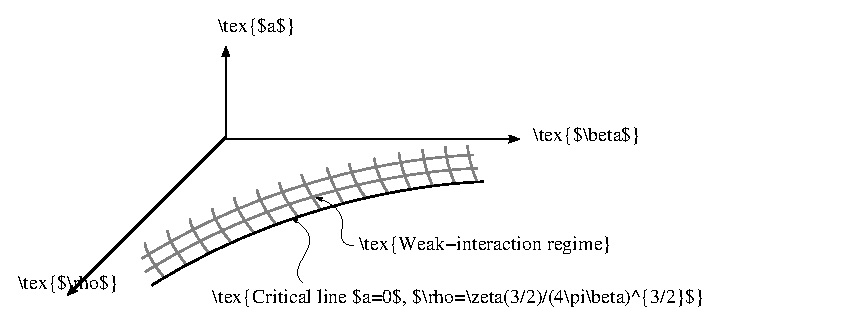
\includegraphics{figures/critical_manifold.eps}
\caption[Short caption for the list of figures.]
	{Here is an EPS file which I put in here and which surely must be
	important.
	\label{fig:important}}
\end{center}
\end{figure}

%% ----------------------------------------------------------------
\section{Section title}
\label{sec:yet_another_section}

The quick brown fox jumped over the lazy dogs.
The quick brown fox jumped over the lazy dogs.
The quick brown fox jumped over the lazy dogs.
The quick brown fox jumped over the lazy dogs.
The quick brown fox jumped over the lazy dogs.
The quick brown \emphidx{fox} jumped over the lazy \emphidx{dogs}.
The quick brown fox jumped over the lazy dogs.
The quick brown fox jumped over the lazy dogs.
The quick brown fox jumped over the lazy dogs.
The quick brown fox jumped over the lazy dogs.
The quick brown fox jumped over the lazy dogs.
The quick brown fox jumped over the lazy dogs.
The quick brown fox jumped over the lazy dogs.

%% ----------------------------------------------------------------
\section{Section title}
\label{sec:last_section}

The quick brown fox jumped over the lazy dogs.
The quick brown fox jumped over the lazy dogs.
The quick brown fox jumped over the lazy dogs.
The quick brown fox jumped over the lazy dogs.
The quick brown fox jumped over the lazy dogs.
The quick brown fox jumped over the lazy dogs.
The quick brown fox jumped over the lazy dogs.
The quick brown fox jumped over the lazy dogs.
The quick brown \plainidx{fox} jumped over the lazy \plainidx{dogs}.
The quick brown fox jumped over the lazy dogs.
The quick brown fox jumped over the lazy dogs.
The quick brown fox jumped over the lazy dogs.
The quick brown fox jumped over the lazy dogs.


\printindex

\chapter{Introduction}
\label{chap:Introduction}

Key information to be included:
\begin{enumerate}
\item outline/organization of the dissertation 
\item Arguments to be made in the dissertation: 
	\begin{enumerate}
	\item To understand language, NLP and Linguistics should work together.
    \item  Gloss is the right `lingua franca' for the two fields.
    \item Linguistics helps NLP.
    \item NLP helps linguistics. 
	\end{enumerate}
\end{enumerate}
\chapter{What are glosses? Why are them golden representations of meanings?}
\label{chap:gloss}

\section{Key Points of The Chapter}
	\begin{enumerate}
	\item Target Audience: CS people
	\item main points:
		\begin{enumerate}
    	\item summary of the Leipzig Glossing Rules \citep{bickel2008leipzig}.  
		\item glossing is the initial processing of the data guided by some specific syntax theory. 
    	\item Glosses contain morphology information (with examples); glosses disambiguate homographs (with many examples); gloss also provide some parsing information because some glosses are determined by structural/constituency context (with examples).       
		\end{enumerate}
 
	\end{enumerate}

\section{Introduction: What are Glosses}

Interlinear Glossed Text (IGT) is widely used in linguistic studies. (\ref{gloss_eg})  is an example of Scottish Gaelic IGT.
\begin{exe}  
\ex\label{gloss_eg} \gll    Tha a athair nas sine na a mh\`athair.\\  
            be.pres 3sm.poss father comp old.cmpr comp 3sm.poss mother
\\  
    \glt    `His father is older than his mother.'  
\end{exe}

(summarize and exemplify the Leipzig Glossing Rules)


\section{The Golden Properties of Glosses}

The most ideal meaning representation system should be built with one-meaning-to-one-representation mappings; in other words, a meaning is mapped to one and only one representation. Natural languages fail to do so, given that synonyms and ambiguous words/phrases are ubiquitous in natural languages. Theoretically, this claim can be tested empirically. Imagine there is a set of special gold meta-linguistic semantic representations, which has the following property: each concept is mapped to one and one representation and each representation is mapped to one and one concept. Given, theses gold representations, it is expected that each gold representation will map to more natural language words than gloss items, and each natural language word will map to more gold representations than gloss items. However, in practice, this is an impossible experiment to conduct, because there are no such gold representation\footnote{It would solve the puzzle of semantics if one should be able to build the set of special golden meta-linguistic semantic representations, and the mappings between the golden representations to natural languages.}. Glosses provide this one-to-one mapping. Second, the gloss data provides hierarchical (non-linear) syntactic parsing information to some degree. 


\subsection{Glosses Cluster Different Words with the Same Meanings}
Gloss collapses words with different forms with the same meanings into a single gloss. In natural languages, the morphology of a word (i.e. the form of a word) may be sensitive to the phonological environments and changing into different forms. Consider the following English example: 
\begin{exe}  
\ex \gll John ate \textbf{an} apple.\\
	John eat.past	\textbf{Det} apple\\
\ex \gll John ate \textbf{a} banana.\\
	John eat.past   \textbf{Det} banana\\
\end{exe}
In the above example, \textit{an} and \textit{a} have the identical meaning\footnote{Semantically, \textit{an} and \textit{a} are existential quantifiers, which declare that a member of a set exists in the world. In formal semantics, \textit{an} and \textit{a} may be defined as follows: $\exists\lambda P[P(x)]$. In the current example, \textit{apple} and \textit{banana} will instantiate $P$ in the formula, and the meanings will be `an apple exists' and `a banana exists'. \citet{kratzer1998semantics} would be a nice introduction for interested readers to see how linguists, specifically semanticians, define, decompose, and compose meanings of languages formally.}. 

\subsection{Glosses disambiguates ambiguous words}
Critically glosses provide `redundant' information. Here `redundant' means that  

\subsection{Glosses are sensitive to hierarchical structure of natural language sentences}
Critically glosses provide `redundant' information. Here `redundant' means that  

\section{What is a Gloss Line}
A gloss line is an artificial sentence using the purified `gloss words'. 

\section{Conclusion} 

% section conclusion (end)
\chapter{Description of the Scottish Gaelic Interlinear Glossed Text Corpus}
\label{chap:Corpus}

	\begin{enumerate}
    \item Original goal of the corpus: a bank of examples of specific syntactic patterns for syntacticians.  
	\item Description of UA Celtic Group's Scottish Gaelic documentation project
    \item Collection of interlinear glossed text data used in syntax paper/dissertations AND language documentation
    \item Auto-glosser and literature on auto-glosser
	\end{enumerate}
\chapter{A Gental Introduction of Machine Learning and Machine Translation}
\label{chap:MT}

	\begin{enumerate}
	\item General review of supervised Machine learning \citep{kotsiantis2007supervised}: The goal is provide a high level of understanding of what machine learning is. Machine Learning is to learn from EXAMPLES/SAMPLES. For example, to define the meaning of `dog', instead of giving all the definable features of `dog', we feed the machine with as many as possible of information of entities of dogs that we have access. Montague Semantics is actually a variant of ML, within which `dog' is defined as `the set of all the dog that exists in the current world.'. As such, Montague Semantics is Machine Learning, because instead of defining 'dog' with certain arbitrary rules (+/- FEATURE), it says 'all the dog entities in the current world'. Definition by samples/examples not by rules.    
	\item Literature on machine translation: from statistical machine translation \citep{koehn2009statistical} to neural machine translation \citep{cho2014learning,cho2014properties,bahdanau2014neural,Koehn_NMT2017}. (Target audience: linguists)
	\end{enumerate}
    
\chapter{Building Translation Systems using Interlinear Glossed Text}
\label{chap:cake}

(

\textbf{Assuming that in the previous chapters the following points are addressed already:}
\begin{itemize}
\item The nature of glosses has been well-explained  (Target audience: CS people without any formal linguistics background):
	\begin{itemize}
	\item What glosses are: A basic intro of interlinear gloss for non-linguists
   \item The golden nature of glosses (encodes NON-LINEAR syntax (i.e. structure parse) and semantics information)
   \item The potential of gloss:	
		\begin{itemize}
		\item potential: providing disambiguation, labeling important grammar morphemes in the source language, providing morphological analysis, providing one-to-many and many-to-one relations of source tokens and target tokens. 
		\end{itemize}
	\end{itemize}
\item A history of machine translation, and a non-mathy description of the methods of doing machine translation. (Target reader: theoretical linguists)
\end{itemize}

               
)


\section{Introduction}
The Innovation is to incorporate the gloss information of Interlinear Glossed Text data into machine translation.

In supervised machine learning models, two factors effects the performance of the trained systems \citep{kotsiantis2007supervised}: a.) the quality of the training data and b.) the choice of the features. The properties of the gloss data as described in *CHAPTERXYZ* make it a better training data than natural language data (Scottish Gaelic in the current case) for the following reasons. First, glosses are more purified that natural language words. The most ideal meaning representation system should be built with one-meaning-to-one-representation mappings; in other words, a meaning is mapped to one and only one representation. Natural languages fail to do so, given that synonyms and ambiguous words/phrases are ubiquitous in natural languages. Glosses provide this one-to-one mapping. Second, the gloss data provides hierarchical (non-linear) syntactic parsing information. To determine what the gloss of a word is, linguists have to look for hierarchical (non-linear) context information. See chapter \ref{chap:gloss} for the discussion on the golden properties of glosses.  

Therefore, theoretically incorporation of the gloss data should improve the translation systems. Specifically, I propose the following hypothesis:
\begin{exe} 
\ex \textbf{Gloss-helps hypothesis: the translation systems trained with the gloss data incorporated should outperform the systems trained with only Gaelic and English sentences pairs (i.e. without gloss data).}

The hypothesis can have two versions, strong and weak:
	\begin{xlist}
	\ex \label{strong_hy} Strong version: Gloss may replace the source natural language totally, and the system outperforms the system trained with source natural language to target language sentence pairs (i.e. the baseline systems).  
	\ex \label{weak_hy} Weak version: Gloss only increases the performance of the baseline systems, but cannot replace the source language.
	\end{xlist}
\end{exe}

The experiments reveal that replacing Gaelic words with glosses doesn't bochoiceost up the performance of the translation systems. Thus, the strong version (replacing-Gaelic-with gloss) of the Gloss-helps hypothesis is not attested. However, it is found that if the Gaelic data and the gloss data are combined in a specific way as the training data, the performance of the systems is improved significantly. 

This chapter describes the experiments conducted to test the Gloss-helps hypothesis and the results attest the weak version.
The rest of the chapter is organized as follows: Section \ref{sec:experimet_setting} describes the constant parameter settings across all the experiments, section \ref{gd_to_gl_to_en} tests the hypothesis in (\ref{strong_hy}), section \ref{gd_plus_gl_to_en} tests the hypothesis in (\ref{weak_hy}),and section 5 concludes the chapter. 

%%%%%%%%%%%%%%%%%%%%%%%%%%%%%%%%%%%%%%%%%%%%%%%%%%%%%%%%%%%%%%%%%%%%%%%%%%%%%%%%%%%%%%%%%

\section{Technical Settings of the Machine Translation Experiments}\label{sec:experimet_setting}
The experiments are conduced by using OpenNMT \citep{2017opennmt}, which implements the state-of-the-art neural net machine translation algorithms \citep{cho2014properties, cho2014learning, bahdanau2014neural}.
The following default hyper-parameter settings of OpenNMT\footnote{See their documentation for the complete default hyper-parameter settings: \url{http://opennmt.net/OpenNMT-py/}.} are used across all models so that the only independent variable is the type of the training data:
\begin{itemize}
\item Word vector size: 500
\item Type of recurrent cell: Long Short Term Memory
\item Number of recurrent layers of the encoder and decoder: 2
\item Number of epochs: 13
\item Size of mini batches: 64
\end{itemize}

The settings of the hyper-parameters do have effects on the performances of the trained models.
A common practice to find the optimal settings of the hyper-parameters is to hold out a subset of the training dataset as the developing dataset, then test the models on the developing data to see what settings are optimal, then merge the developing dataset and training dataset as a new training set, and then train on this new training set using the found optimal hyper-parameters.

However, given that finding the optimal settings of the hyper-parameters is not relevant to our research and causing unnecessary complications, the process of optimizing the settings of the hyper-parameters is not implemented, and I simply adopt OpenNMT's default settings. The employed settings of the hyper-parameters should be viewed as arbitrarily chosen, and there are room to tune the models for better performance. Critically, these settings are viewed as constants, so that we can focus on the effects of different treatments on the source sequences in the translation experiments.

The data and the scripts will be accessible on GitHub\footnote{\url{https://github.com/lucien0410/Scottish_Gaelic}}, so that the results can be reproduced.  

\section{Gloss Representation Solely Does NOT Outperform Gaelic Sentences} \label{gd_to_gl_to_en}
This section tests the strong version of Gloss-helps hypothesis in (\ref{strong_hy}).
Given the assumption that gloss may be better than any natural language in terms of representing meanings, it is expected that for neural net machine translation systems it is easier to learn how to translate from the glosses of Scottish Gaelic to English than to learn how to translate from Scottish Gaelic to English. However, the results show that there is no significance difference between the two types of data (i.e. GLOSS $\rightarrow$ English and Gaelic $\rightarrow$ English).

\subsection{Procedure of the Experiments}
I use repeated random sub-sampling validation to compare the performances of the two type of models.

Totally we have 8,388 indexed 3-tuples of Gaelic sentence, a gloss line and an English translation. In the interlinear glossed text example below, each line is an argument of a 3-tuple sample.

\begin{exe} 
\ex \gll    Tha a athair nas sine na a mh\`athair.\\ 
           be.pres 3sm.poss father comp old.cmpr comp 3sm.poss mother
\\ 
   \glt    `His father is older than his mother.' 
\end{exe}

The 3-tuple representation of the above example is:
\begin{exe}
\ex <``Tha a athair nas sine na a mh\`athair'', ``be.pres 3sm.poss father comp old.cmpr comp 3sm.poss mother'', ``His father is older than his mother''>
\end{exe}

First, the samples (i.e. the 3-tuples) are randomly split into three datasets: training set (N=6,388), validation set (N=1,000), and test set (N=1,000)\footnote{Here the random sampling process is achieved by using the \begin{myfont}random.sample(population, k)\end{myfont} function in the standard library of python.}.

\begin{exe}
\ex Definitions of datasets:\\
	Let:
	\begin{xlist}
	\ex 	Index\textsubscript{Train}, Index\textsubscript{Validation}, and Index\textsubscript{Test} be sets of random indexes from 0 to 8,387.
   \ex		Index\textsubscript{Train} $\cap$ Index\textsubscript{Validation} $\cap$ Index\textsubscript{Test} = $\emptyset$
   \ex 	|Index\textsubscript{Train}| = 6,388; |Index\textsubscript{Validation}| = 1,000; |Index\textsubscript{Test}| = 1,000.
   \end{xlist}
\end{exe}
The step above just randomly splits the indexes of the 3-tuples into three distinct sets: Index\textsubscript{Train}, Index\textsubscript{Validation}, and Index\textsubscript{Test}. Based on the indexes, we generate the sets of samples. For each index, the 3-tuple is split into two pairs: <gloss, English>, <Gaelic, English>, so that later we can compare the different effects of gloss lines and Gaelic sentences. For each pair, the first item is the source sequence, and the second item is the target sequence. The systems learns how to map the source sequence to the target sequence.   

\begin{exe}
	\ex Gloss to English
		\begin{xlist}
		\ex \label{GLOSStoENTrain} GLOSStoEN\textsubscript{Train}   = $\{<gloss_i,En_i>  \mid i \in Index\textsubscript{Train} \}$ \\
		\ex \label{GLOSStoENVal} GLOSStoEN\textsubscript{Validation}   = $\{<gloss_i,En_i>  \mid i \in Index\textsubscript{Validation} \}$ \\
		\ex \label{GLOSStoENTest}GLOSStoEN\textsubscript{Test} = $\{<gloss_i,En_i>  \mid i \in Index\textsubscript{Test} \}$ \\
		\ex  Example: <``be.pres 3sm.poss father comp old.cmpr comp 3sm.poss mother'', ``His father is older than his mother.''>
		\end{xlist}

	
	\ex Gaelic to English
		\begin{xlist}
		\ex \label{GDtoENTrain} GDtoEN\textsubscript{Train}   = $\{<GD_i,En_i>  \mid i \in Index\textsubscript{Train} \}$ \\
		\ex \label{GDtoENVal} GDtoEN\textsubscript{Validation}   = $\{<GD_i,En_i>  \mid i \in Index\textsubscript{Validation} \}$ \\
		\ex \label{GDtoENTest} GDtoEN\textsubscript{Test}    = $\{<GD_i,En_i>  \mid i \in Index\textsubscript{Test} \}$ \\
		\ex Example: <``Tha a athair nas sine na a mh\`athair.'', ``His father is older than his mother.''>
		\end{xlist}
\end{exe}
The models are trained with the training set and validation set (i.e. the model learns how to map the source sequence to the target sequence). Both training set and validation set are known information for the models\footnote{Technically speaking, the validation set is part of the training data in terms of machine learning. The presence of the validation set is a special requirement of neural net machine learning, which uses the validation set to evaluate the convergence of the training.}. Specifically, the neural net system learns how to maps gloss lines to English sentences from samples in (\ref{GLOSStoENTrain}) and (\ref{GLOSStoENVal}), and another neural net system learns how to maps Gaelic sentences to English sentences from from samples in (\ref{GDtoENTrain}) and (\ref{GDtoENVal}).

\begin{exe}
\ex Models:
	\begin{xlist}
	\ex \label{ModelGlossToEN} Model\textsubscript{GLOSStoEN} = Model trained with GLOSStoEN\textsubscript{Train} in (\ref{GLOSStoENTrain}) and GLOSStoEN\textsubscript{Validation} in (\ref{GLOSStoENVal})
	\ex \label{ModelGDToEN}Model\textsubscript{GDtoEN} = Model trained with GDtoEN\textsubscript{Train} in (\ref{GDtoENTrain}) and GDtoEN\textsubscript{Validation} in (\ref{GDtoENVal})
	\end{xlist}	
\end{exe}
The two trained models (gloss-to-English and Gaelic-to-English) then take the right source sequences of the test sets (i.e. glossing lines and Gaelic sentences for Model\textsubscript{GLOSStoEN} and Model\textsubscript{GDoEN} respectively) as inputs and then generate the predicted target sequences (i.e. English sentences).

\begin{exe}
\ex Predictions:
	\begin{xlist}
	\ex Predictions\textsubscript{GLOSStoEN} = A list of English sequences that Model\textsubscript{GLOSStoEN} maps to from the gloss sequences in (\ref{GLOSStoENTest})
	\ex Predictions\textsubscript{GDtoEN} = A list of English sequences that Model\textsubscript{GDtoEN} maps to from the Gaelic sentences in (\ref{GDtoENTest})
	\end{xlist}	
\end{exe}

To evaluate the model, the predicted target sequences are checked against the target sequences of the test set (i.e. the gold standard/human-translated English sentences).
Specifically, the BLEU (bilingual evaluation understudy)\footnote{There are other automatic machine translation evaluation algorithms available, such as translation edit rate \citep{Snover06astudy} and Damerau-Levenshtein edit distance \citep{damerau1964technique, levenshtein1966binary}. BLEU is chosen for the current experiments because it is the most widely used evaluation algorithm, and the correlation between the BLUE score evaluation and human judgment evaluation is also well-acknowledged.} score metric \citep{bleu} of each prediction is calculated using the \begin{myfont} multi-bleu.perl\end{myfont}\footnote{The script can be downloaded from: \url{https://github.com/moses-smt/mosesdecoder/blob/master/scripts/generic/multi-bleu.perl}}
script, a public implementation of Moses \citep{moses}. The BLEU score calculation is an automatic evaluation of how similar two copora are. In the current experiments we are comparing the predicted target sequences with the gold standard. The BLEU score of 100 means the two copora are identical, and the BLEU score of 0 means the two copora are completely distinct from each other.

\begin{exe}
\ex Gold-Standard = English sentences in (\ref{GLOSStoENTest}) = English sentences in (\ref{GDtoENTest})
\end{exe}
Note that the gold-standard is the same because they are the same English sentences in the 3-tuples samples. Then the two sets of predicted English sentences are evaluated, yielding two BLEU scores.  

\begin{exe}
\ex Scores: \\
 \begin{xlist}
	\ex Score\textsubscript{GLOSStoEN} = BLEU(Gold-Standard, Predictions\textsubscript{GLOSStoEN}) \\
	\ex Score\textsubscript{GDtoEN} = BLEU(Gold-Standard, Predictions\textsubscript{GDtoEN}) \\
 \end{xlist}
\end{exe}
This procedure of splitting the data into three sub-sets, training the models, and evaluating the models is executed for ten times.

\subsection{Result} \label{gdglen_results}
After ten rounds of repeated random sub-sampling validation, ten pairs of scores of the two models are generated, as shown in the following table.
% !Rnw root = cake_chapter.Rnw
% latex table generated in R 3.4.4 by xtable 1.8-2 package
% Wed Apr  4 13:20:48 2018
\begin{table}[ht]
\centering
\begin{tabular}{lcc}
  \hline
Round & Gaelic (Baseline) & GLOSS \\ 
  \hline
0 & 17.29 & 18.39 \\ 
  1 & 16.42 & 18.00 \\ 
  2 & 15.29 & 16.02 \\ 
  3 & 15.97 & 20.22 \\ 
  4 & 17.79 & 19.02 \\ 
  5 & 16.73 & 15.53 \\ 
  6 & 17.11 & 18.00 \\ 
  7 & 16.37 & 20.08 \\ 
  8 & 15.93 & 15.82 \\ 
  9 & 16.99 & 15.93 \\ 
   \hline
Mean & 16.59 & 17.70 \\ 
   \hline
\end{tabular}
\caption{BLEU scores of Model\textsubscript{GDtoEN} and Model\textsubscript{GLOSStoEn}} 
\label{Table:GLOSS}
\end{table}
The average score of the Models\textsubscript{GLOSStoEN} is only sightly higher than the average score of the Models\textsubscript{GDtoEN}.
Also, after doing a paired T-test, the difference between the two types of models is not attested
(M\textsubscript{GDToEn}=16.59, SD\textsubscript{GDToEn}=0.74; M\textsubscript{GLOSStoEN}=17.70, SD\textsubscript{GLOSStoEN}=1.78; t(9)=1.97, p=0.080)

\subsection{Summary}
The ultimate practical goal of the dissertation is to use glossing data to develop better machine translation systems. Here \textit{better} means to be better than a baseline system, which is the machine translation system trained with Gaelic-to-English translation samples. The models in (\ref{ModelGDToEN}) are the baseline systems, and their scores are in the Gaelic column of table (\ref{Table:GLOSS}). These are the target scores that we aims to outperform. The experiment above is the first attempt to improve that scores by using the \textit{gloss treatment}, in which the Gaelic sentences are replaced with gloss lines.  However, the result shows that this \textit{gloss treatment} is not effective as the scores of the gloss models are not statistically higher than the baseline Gaelic-to-English models. 

\subsection{Discussion}
It is assumed that the performances of the machine translation systems are correlated with the quality of the representation of meanings in the source sequences. Better representations of meanings yield better machine translation systems. Given the results in (\ref{gdglen_results}) that the gloss models are not better than the Gaelic models, it is concluded that glosses and natural languages are equally good in terms of representing meanings. The strong version of the Gloss-helps hypothesis does not hold.

There are several remarks that need to make for the current result. First, the result falsifies the point of view about glosses in chapter (\ref{chap:gloss}) that the gloss line is a golden semantic representation hand-crafted by linguists.
It turns that this artificial language, the gloss lines, is only marginal better than Gaelic, as the mean BLEU score of the gloss treatment is slightly higher than that of the baseline systems. This can be viewed as an evidence of language evolution.
The written form of a natural language is actually already optimized for representing semantics to the same degree of gloss line representations.
Second, if we want to actually apply the gloss treatment to translate a Gaelic sentence to English, we encounter an immediate problem. The actual source sequence is a Gaelic sentence, while the required source sequence for the gloss treatment is a gloss line. The auto-glosser described in chapter (\ref{chap:gloss}) may convert the Gaelic sentence to a gloss line, but the conversion is not perfect at all. Given this, even if the gloss treatment should work, it is not practical unless we may convert Gaelic sentence to gloss line perfectly.      

We may now combine Gaelic and Gloss sentences as the training data to test the weak version of the Gloss-helps hypothesis. The experiments and results are reported in the next chapter.
%%%%%%%%%%%%%%%%%%%%%%%%%%%%%%%%%%%%%%%%%%%%%%%%%%%%%%%%%%%%%%%%%%%%%%%%%%%%%%%%%%%%%%%%%%%
\chapter{Combining Gaelic Words with Glosses}\label{gd_plus_gl_to_en}
\section{Introduction}
In the previous section, we attempt to build a system by using the \textit{gloss treatment} to outperform the baseline system. It turns that using gloss line solely is not effective enough to improve the system. However, this result does not falsify the gloss-helps hypothesis; instead, it indicates that combination of the gloss line data and the Gaelic sentence data is necessary. In other words, the questions now are: 
\begin{exe}
	\ex 
	\begin{xlist}
		\ex Does adding the gloss data into the Gaelic data will improve the translation system? 
		\ex If yes, what are the right ways of blending these two types of meaning representations together? 
	\end{xlist}	
\end{exe}

This section reports various ways of combining the gloss line data and the Gaelic sentence data, and the experiments and their results using these different treatments. Critically, a specific way of combining Gloss data and Gaelic date (termed as `\textit{Parallel-Partial}' treatment) boosts the performance significantly. The model trained with this specially arranged training data also significantly outperforms Google's Gaelic-to-English translation system.

In this section, I will first describe the most effective treatment, termed as `\textit{Parallel-Partial}' treatment, and the results, and then I will report the experiments done with other relevant logical treatments (i.e. other ways of combining glossing data and Gaelic data). 

\section{The `Parallel-Partial' Treatment Outperforms Any Other Treatments and the Baseline Significantly}

\subsection{Data Preprocessing Using the Parallel-Partial Treatment}
The Parallel-Partial treatment uses the training and validation data of the baseline system and that of the gloss treatment system.  
The training and validation data of the baseline system are pairs of a Gaelic sentence and a English sentences (see (\ref{GDtoENTrain}) and (\ref{GDtoENVal}) ), 
and the data of the gloss treatment are pairs of a gloss line and a English sentences (see (\ref{GLOSStoENTrain}) and (\ref{GLOSStoENVal}). 
These two groups of data are combined in a parallel manner in the current treatment. Now the size of training set and validation set is doubled. In the baseline system and the gloss treatment system, we have 6,388 samples in the training set and 1,000 samples in the validation set. The current treatment has 12,776 samples in the training set and 2,000 samples in the validation set. This is the \textit{parallel} part of the treatment. 

Additionally, I utilize the alignment property between the Gaelic word and the gloss to further build pairs of a Gaelic word and a gloss. These pairs are also included into the training set and validation set of the current treatment. This is the \textit{partial} part of the treatment.   

For concreteness, consider the following interlinear glossed text: 
\begin{exe}  
\ex \gll    Tha a athair nas sine na a mh\`athair.\\  
            be.pres 3sm.poss father comp old.cmpr comp 3sm.poss mother\\  
    \glt    `His father is older than his mother.'  
\end{exe}

With the interlinear glossed text, the parallel treatment will generate two pairs of samples:

\begin{exe}
	\ex
	\begin{xlist}
		\ex Gaelic to English: \\<``Tha a athair nas sine na a mh\`athair'', ``His father is older than his mother.''>
		\ex Gloss to English: \\<``be.pres 3sm.poss father comp old.cmpr comp 3sm.poss mother'', ``His father is older than his mother''>
	\end{xlist}
\end{exe}

The partial treatment then generates pairs of a Gaelic word and a gloss token: 
\begin{exe}
	\ex
	\begin{xlist}
		\ex <``Tha'', ``be.pres''>
		\ex <``a'', ``3sm.poss''>
		\ex <``athair'', ``father''>
		\ex <``nas'', ``comp''>
		\ex <``sine'', ``old.cmpr''>
		\ex <``na'', ``comp''>
		\ex <``a'', ``3sm.poss''>
		\ex <``mh\`athair'', ``mother''>
	\end{xlist}
\end{exe}

\subsection{Results of the Parallel-Partial Treatment}

With the training and validation data ready, now we can train models and evaluate them. Critically, the same technical settings and the same test sets in the previous experiments are used, and the same procedures are executed. The only difference is the training and validation data. As shown in the following table, the Parallel-Partial treatment has a tremendous effect in improving the baseline system.        

% !Rnw root = cake_chapter.Rnw
% latex table generated in R 3.4.4 by xtable 1.8-2 package
% Wed Apr  4 13:20:48 2018
\begin{table}[ht]
\centering
\begin{tabular}{lcc}
  \hline
Round & Gaelic (Baseline) & ParaPart \\ 
  \hline
0 & 17.29 & 32.64 \\ 
  1 & 16.42 & 32.28 \\ 
  2 & 15.29 & 29.94 \\ 
  3 & 15.97 & 31.18 \\ 
  4 & 17.79 & 32.83 \\ 
  5 & 16.73 & 31.11 \\ 
  6 & 17.11 & 32.19 \\ 
  7 & 16.37 & 33.52 \\ 
  8 & 15.93 & 30.93 \\ 
  9 & 16.99 & 34.35 \\ 
   \hline
Mean & 16.59 & 32.10 \\ 
   \hline
\end{tabular}
\caption{BLEU scores of Model\textsubscript{GDtoEN} and Model\textsubscript{ParaParttoEn}} 
\label{Table:ParaPart}
\end{table}
The first and the second columns are BLUE scores of the baseline systems and the systems with the Parallel-Partial treatment respectively. The latter is significantly better than the former
(M\textsubscript{GDToEn}=16.59, SD\textsubscript{GDToEn}=0.74; M\textsubscript{ParaPart}=32.10, SD\textsubscript{ParaPart}=1.33; t(9)=48.95, p<0.01).
The comparison of the average BLUE scores of the groups of systems shows that the Parallel-Partial treatment improves the performance of the baseline system for 93 percent.
%(M\textsubscript{GDToEn}=16.59, SD\textsubscript{GDToEn}=0.74; M\textsubscript{ParaPart}=32.10, SD\textsubscript{ParaPart}=1.33,; t(9)=48.95, p<0.010.000).


%%%%%%%%%%%%%%%%%%%%%%%%%%%%%%%%%%%%
\section{Other Possible Treatments}
This section reports other possible ways of blending the Gaelic sentences and gloss lines. However, all of these treatments are not as effective as the Parallel-Partial treatment. Again, the same procedure and the same test datasets are used across all the experiments.    

\subsection{The Parallel Treatment}\label{treatment:Para}
\subsubsection{Method of the Parallel Treatment}
The Parallel treatment is using the parallel part of the Parallel-Partial treatment. With this treatment, a chunk of interlinear glossed text is split into two pairs. For example, the chunk of interlinear glossed text in (\ref{igt}) becomes two samples in (\ref{sample_pair}): 
\begin{exe} 
\ex \label{igt}
	\gll    Tha a athair nas sine na a mh\`athair.\\  
            be.pres 3sm.poss father comp old.cmpr comp 3sm.poss mother \\
    \glt    `His father is older than his mother.'  
\end{exe}


\begin{exe} 
	\ex \label{sample_pair}
	\begin{xlist}
		\ex Gaelic to English: \\<``Tha a athair nas sine na a mh\`athair'', ``His father is older than his mother.''>
		\ex Gloss to English: \\<``be.pres 3sm.poss father comp old.cmpr comp 3sm.poss mother'', ``His father is older than his mother''>
	\end{xlist}
\end{exe}

\subsubsection{Results of the Parallel Treatment}\label{treatment:Para_result}
% !Rnw root = cake_chapter.Rnw
% latex table generated in R 3.4.4 by xtable 1.8-2 package
% Wed Apr  4 13:20:48 2018
\begin{table}[ht]
\centering
\begin{tabular}{lcc}
  \hline
Round & Gaelic (Baseline) & Para \\ 
  \hline
0 & 17.29 & 25.42 \\ 
  1 & 16.42 & 25.32 \\ 
  2 & 15.29 & 20.72 \\ 
  3 & 15.97 & 22.22 \\ 
  4 & 17.79 & 24.27 \\ 
  5 & 16.73 & 24.55 \\ 
  6 & 17.11 & 27.03 \\ 
  7 & 16.37 & 25.34 \\ 
  8 & 15.93 & 24.24 \\ 
  9 & 16.99 & 25.96 \\ 
   \hline
Mean & 16.59 & 24.51 \\ 
   \hline
\end{tabular}
\caption{BLEU scores of Model\textsubscript{GDtoEN} and Model\textsubscript{ParatoEn}} 
\label{Table:Para}
\end{table}The table in (\ref{Table:Para}) compares the performances of this treatment and the baseline. Critically, the Parallel treatment is effective in improving the baseline systems (M\textsubscript{GDToEn}=16.59, SD\textsubscript{GDToEn}=0.74; M\textsubscript{Para}=24.51, SD\textsubscript{Para}=1.84; t(9)=17.50, p < 0.01). 
% !Rnw root = cake_chapter.Rnw
%GDParaParaPart1_table.Rnw does NOT print out anything but just load the sexpr variables 
However, the best treatment (i.e. the Parallel-Partial treatment) is still far better than this Parallel treatment 
(M\textsubscript{Para}=24.51, SD\textsubscript{Para}=1.84; M\textsubscript{ParaPart}=32.10, SD\textsubscript{ParaPart}=1.33; t(9)=18.73, p < 0.01 ).
% !Rnw root = cake_chapter.Rnw
% latex table generated in R 3.4.4 by xtable 1.8-2 package
% Wed Apr  4 13:20:48 2018
\begin{table}[ht]
\centering
\begin{tabular}{lccc}
  \hline
Round & Gaelic (Baseline) & Para & ParaPart \\ 
  \hline
0 & 17.29 & 25.42 & 32.64 \\ 
  1 & 16.42 & 25.32 & 32.28 \\ 
  2 & 15.29 & 20.72 & 29.94 \\ 
  3 & 15.97 & 22.22 & 31.18 \\ 
  4 & 17.79 & 24.27 & 32.83 \\ 
  5 & 16.73 & 24.55 & 31.11 \\ 
  6 & 17.11 & 27.03 & 32.19 \\ 
  7 & 16.37 & 25.34 & 33.52 \\ 
  8 & 15.93 & 24.24 & 30.93 \\ 
  9 & 16.99 & 25.96 & 34.35 \\ 
   \hline
Mean & 16.59 & 24.51 & 32.10 \\ 
   \hline
\end{tabular}
\caption{BLEU scores of Model\textsubscript{GDtoEN}, Model\textsubscript{ParatoEN} and Model\textsubscript{ParaParttoEN} } 
\label{Table:Concating}
\end{table}
\subsection{Interleaving Gaelic Words and Gloss Items And Concating them}\label{treatment:InterleavingAndConCat}
\subsubsection{Method of the Interleaving Treatment}
Instead of putting the pairs of a Gaelic sentence and a English sentences and the pairs of a gloss line and a English sentence in a parallel manner, we may just literally blend a Gaelic sentence and a gloss line by interleaving them. Consider the following example:

\begin{exe} 
\ex 
	\begin{xlist}
	\ex \label{ex_interleave:in}
		\gll	 Tha a athair nas sine na a mh\`athair.\\  
     		     be.pres 3sm.poss father comp old.cmpr comp 3sm.poss mother \\
    	\glt    `His father is older than his mother.'  

    \ex \label{ex_interleave:out} <``Tha be.pres a 3sm.poss athair father nas comp sine old.cmpr na comp a 3sm.poss mh\`athair mother'', ``His father is older than his mother''>
    \end{xlist}
\end{exe}

Given the chuck of interlinear glossed text data in (\ref{ex_interleave:in}), the Interleaving treatment generates the sample in (\ref{ex_interleave:out}).  
The results are given in the following table. 
% !Rnw root = cake_chapter.Rnw
% latex table generated in R 3.4.4 by xtable 1.8-2 package
% Wed Apr  4 13:20:48 2018
\begin{table}[ht]
\centering
\begin{tabular}{lcc}
  \hline
Round & Gaelic (Baseline) & interleavingGdGLOSS \\ 
  \hline
0 & 17.29 & 13.67 \\ 
  1 & 16.42 & 12.49 \\ 
  2 & 15.29 & 11.01 \\ 
  3 & 15.97 & 12.33 \\ 
  4 & 17.79 & 12.56 \\ 
  5 & 16.73 & 12.13 \\ 
  6 & 17.11 & 11.55 \\ 
  7 & 16.37 & 12.78 \\ 
  8 & 15.93 & 12.43 \\ 
  9 & 16.99 & 11.65 \\ 
   \hline
Mean & 16.59 & 12.26 \\ 
   \hline
\end{tabular}
\caption{BLEU scores of Model\textsubscript{GDtoEN} and Model\textsubscript{interleavingGdGLOSStoEn}} 
\label{Table:interleavingGdGLOSS}
\end{table}\newline
It turns out this treatment has a significant negative effect
(M\textsubscript{GDToEn}=16.59, SD\textsubscript{GDToEn}=0.74; M\textsubscript{interleavingGdGLOSS}=12.26, SD\textsubscript{interleavingGdGLOSS}=0.74,; t(9)=-17.06, p=0.000). This is not the right way of incorporating gloss line data. 


\subsubsection{Method of Concating Gaelic Words and Gloss Words }\label{treatment:Concating}
A quick and close amendment of the Interleaving approach is to concatenate the aligned Gaelic word and gloss item as a single token. Given the same chunk of interlinear glossed text data, this treatment generates the following sample:

\begin{exe} 
\ex 
	\begin{xlist}
	\ex 
		\gll	 Tha a athair nas sine na a mh\`athair.\\  
     		     be.pres 3sm.poss father comp old.cmpr comp 3sm.poss mother \\
    	\glt    `His father is older than his mother.'  

    \ex <``Tha\_be.pres a\_3sm.poss athair\_father nas\_comp sine\_old.cmpr na\_comp a\_3sm.poss mh\`athair\_mother'', ``His father is older than his mother''>
    \end{xlist}
\end{exe}

\subsubsection{Results of Concating Gaelic Words and Gloss Words}
The performances of this treatment is given in the following table.
% !Rnw root = cake_chapter.Rnw
% latex table generated in R 3.4.4 by xtable 1.8-2 package
% Wed Apr  4 13:20:48 2018
\begin{table}[ht]
\centering
\begin{tabular}{lcc}
  \hline
Round & Gaelic (Baseline) & ConcatGLOSSGaelic \\ 
  \hline
0 & 17.29 & 15.42 \\ 
  1 & 16.42 & 14.31 \\ 
  2 & 15.29 & 15.38 \\ 
  3 & 15.97 & 14.18 \\ 
  4 & 17.79 & 18.63 \\ 
  5 & 16.73 & 14.89 \\ 
  6 & 17.11 & 15.16 \\ 
  7 & 16.37 & 15.20 \\ 
  8 & 15.93 & 15.50 \\ 
  9 & 16.99 & 15.72 \\ 
   \hline
Mean & 16.59 & 15.44 \\ 
   \hline
\end{tabular}
\caption{BLEU scores of Model\textsubscript{GDtoEN} and Model\textsubscript{ConcatGLOSSGaelictoEn} } 
\label{Table:Concating}
\end{table}\newline
The result shows that this treatment hurts the baseline systems badly instead of improving them (M\textsubscript{GDToEn}=16.59, SD\textsubscript{GDToEn}=0.74; M\textsubscript{ConcatGLOSSGaelic}=15.44, SD\textsubscript{ConcatGLOSSGaelic}=1.23,; t(9)=-3.64, p=0.010).

%%%%%%%%%%
\subsection{Hybrid: Gaelic or Gloss}
\subsubsection{Method of Hybrid}
The Hybrid treatment aims to reduce the potential lexical ambiguity. A Gaelic word may maps to multiple gloss, and a glosses may maps to multiple Gaelic words. Let's assume a toy chunk of interlinear glossed text data (a one-word sentence): 

\begin{exe} 
\ex 
	\gll	 Gaelic\_word\\  
     		 Gloss\_item \\
    \glt    English translation  
\end{exe} 

Now we aim to build a single sample that is either <Gaelic\_word, English translation > or <Gloss\_item, English translation >. The criterion is which one, the Gaelic word or the gloss item, is less ambiguous. The less ambiguous one is the winner. For example, if the Gaelic word is potentially mapped to 10 glosses and if the gloss item is potentially mapped 2 Gaelic word, then <Gloss\_item, English translation> is chosen; other the other hand if the ambiguity situation is reverted, then <Gaelic\_word, English translation > is chosen. However, when the situation is tight (i.e. both the Gaelic word and gloss item are equally ambiguous), a default setting is needed to be chosen. The choices of the default setting split this single treatment into two treatments: default as Gaelic or default as gloss.
\subsubsection{Result of Hybrid}    
% !Rnw root = cake_chapter.Rnw
% latex table generated in R 3.4.4 by xtable 1.8-2 package
% Wed Apr  4 13:20:48 2018
\begin{table}[ht]
\centering
\begin{tabular}{lcc}
  \hline
Round & Gaelic (Baseline) & HybridDefaultAsGaelic \\ 
  \hline
0 & 17.29 & 9.44 \\ 
  1 & 16.42 & 9.07 \\ 
  2 & 15.29 & 7.69 \\ 
  3 & 15.97 & 9.12 \\ 
  4 & 17.79 & 9.08 \\ 
  5 & 16.73 & 10.45 \\ 
  6 & 17.11 & 8.62 \\ 
  7 & 16.37 & 10.00 \\ 
  8 & 15.93 & 10.52 \\ 
  9 & 16.99 & 8.46 \\ 
   \hline
Mean & 16.59 & 9.24 \\ 
   \hline
\end{tabular}
\caption{BLEU scores of Model\textsubscript{GDtoEN} and Model\textsubscript{HybridDefaultAsGaelictoEn}} 
\label{Table:HybridDefaultAsGaelic}
\end{table}When the default setting is the Gaelic word, the performances are significantly worse than than the baseline systems, as shown in table (\ref{Table:HybridDefaultAsGaelic}).  
(M\textsubscript{GDToEn}=16.59, SD\textsubscript{GDToEn}=0.74; M\textsubscript{ReplacingGaelic}=9.24, SD\textsubscript{ReplacingGaelic}=0.89,; t(9)=-21.03, p < 0.01).
% !Rnw root = cake_chapter.Rnw
% latex table generated in R 3.4.4 by xtable 1.8-2 package
% Wed Apr  4 13:20:48 2018
\begin{table}[ht]
\centering
\begin{tabular}{lcc}
  \hline
Round & Gaelic (Baseline) & HybridDefaultAsGLOSS \\ 
  \hline
0 & 17.29 & 15.95 \\ 
  1 & 16.42 & 15.60 \\ 
  2 & 15.29 & 14.15 \\ 
  3 & 15.97 & 14.72 \\ 
  4 & 17.79 & 15.74 \\ 
  5 & 16.73 & 14.88 \\ 
  6 & 17.11 & 14.45 \\ 
  7 & 16.37 & 16.41 \\ 
  8 & 15.93 & 15.15 \\ 
  9 & 16.99 & 17.61 \\ 
   \hline
Mean & 16.59 & 15.47 \\ 
   \hline
\end{tabular}
\caption{BLEU scores of Model\textsubscript{GDtoEN} and Model\textsubscript{HybridDefaultAsGLOSS}} 
\label{Table:HybridDefaultAsGLOSS}
\end{table}When the default setting is the Gaelic word, the performances are sightly worse than than the baseline systems, as shown in table (\ref{Table:HybridDefaultAsGLOSS}).
(M\textsubscript{GDToEn}=16.59, SD\textsubscript{GDToEn}=0.74; M\textsubscript{ReplacingGaelic}=15.47, SD\textsubscript{ReplacingGaelic}=1.03,; t(9)=-3.67, p < 0.01 ).


\section{Summary and Conclusion}
The chapter reports machine translation experiments that aims to find how the gloss line information can improve the performance of the baseline Gaelic-to-English translation systems. It is found that the Parallel-Partial is highly effective. The complete BLEU scores of various treatments are given in the following table. 
% latex table generated in R 3.4.4 by xtable 1.8-2 package
% Wed Apr  4 13:20:48 2018
\begin{table}[ht]
\centering
\begin{tabular}{lrrrrrrrr}
  \hline
Round & Baseline & GLOSS & ParaPart & Para & Interleaving & Concat & HybrGaelic & HybrGLOSS \\ 
  \hline
0 & 17.29 & 18.39 & 32.64 & 25.42 & 13.67 & 15.42 & 9.44 & 15.95 \\ 
  1 & 16.42 & 18.00 & 32.28 & 25.32 & 12.49 & 14.31 & 9.07 & 15.60 \\ 
  2 & 15.29 & 16.02 & 29.94 & 20.72 & 11.01 & 15.38 & 7.69 & 14.15 \\ 
  3 & 15.97 & 20.22 & 31.18 & 22.22 & 12.33 & 14.18 & 9.12 & 14.72 \\ 
  4 & 17.79 & 19.02 & 32.83 & 24.27 & 12.56 & 18.63 & 9.08 & 15.74 \\ 
  5 & 16.73 & 15.53 & 31.11 & 24.55 & 12.13 & 14.89 & 10.45 & 14.88 \\ 
  6 & 17.11 & 18.00 & 32.19 & 27.03 & 11.55 & 15.16 & 8.62 & 14.45 \\ 
  7 & 16.37 & 20.08 & 33.52 & 25.34 & 12.78 & 15.20 & 10.00 & 16.41 \\ 
  8 & 15.93 & 15.82 & 30.93 & 24.24 & 12.43 & 15.50 & 10.52 & 15.15 \\ 
  9 & 16.99 & 15.93 & 34.35 & 25.96 & 11.65 & 15.72 & 8.46 & 17.61 \\ 
   \hline
Mean & 16.59 & 17.70 & 32.10 & 24.51 & 12.26 & 15.44 & 9.24 & 15.47 \\ 
   \hline
\end{tabular}
\caption{BLEU scores of the treatments} 
\label{table:complete_table}
\end{table}
The aim of chapter is to report and document how the experiments are done and what the results are. This is merely reporting the linguist and non-linguistic facts. The implications and relevant works in the literature will be discussed in the next chapter.   


(
Hi Mike: 
The current chapter reports the what are done and how (i.e. the fact);
the next chapter I will discuss the why questions, and discuss similar works in the literature.  

)
% \subsection{literature}

% what about \ref{Table:interleavingGdGLOSS} \ref{table:complete_table}
% Linguistics-informed MT: \citep{sennrich2016linguistic}\\ 

% Multi-task Sequence to Sequence Learning: \citep{luong2015multi}\\
% what is Multi-task learning:  \citep{Overview_Multi-Task_Learning}\\
% add ccc to target seq: \citep{ccg_target_seq}\\
% google zero shot: \citep{google_zero_shot}\\
\chapter{Interlinear Glossed Text Data In Other Languages}
\label{chap:gloss_in_other_languages}

To run the same experiments on Online Database of Interlinear Text \citep{ODIN, Xia2016} to show that incorporating gloss information works effectively across different languages.  
\chapter{Implications on Theoretical Linguistics}
\label{chap:Implications_ling}
\chapter{Conclusion}
Conclusion


\bibliographystyle{te}

\bibliography{ref}

%% ================================================================
\end{document}
